\section{Einleitung} % (fold)
    \label{sec:einleitung}
    \dots Wissenschaftlicher Kontext, zufällige Ähnlichkeit in Alignments \dots

    Diese Bachelorarbeit beinhaltet die Entwicklung von Version 0.4 des Projekts \protfin\footnote{\url{https://github.com/usadellab/prot-fin/releases/tag/v0.4/experiments/recog_with_fft} bei Commit \href{https://github.com/usadellab/prot-fin/tree/86ea260b7c6d7bb520b57e2b29e350bd3942fe71/experiments/recog_with_fft}{\texttt{86ea260}}} und den zugehörigen Experimenten. \protfin\ stellt sich dem Problem zufälliger Ähnlichkeit und beschäftigt sich daher mit der Frage, ob es möglich ist, funktionsähnliche Proteine über ihre physikalischen Eigenschaften zu identifizieren, anstelle der lediglichen Buchstaben ihrer Aminosäuren, und ob das die Problematik umgeht.

    Eine Grundlage hierfür bildet die Arbeit von Akinori Kidera \textit{et. al.}, welcher in seiner Forschungsgruppe mittels statistischer Faktorenanalyse 188 physikalische Eigenschaften der 20 natürlich vorkommenden Aminosäuren auf lediglich 10 sogenannte Kidera-Faktoren reduziert hat, die zusammen all diese Eigenschaften am besten erklären \vgl{kidera}. So ist beispielsweise die Hydrophobizität ein ebensolcher Faktor, da diese mit vielen anderen Eigenschaften stark in Korrelation steht.

    Der Einfluss eines jeden Faktors in einer Aminosäure lässt sich numerisch darstellen, sodass eine Aminosäuresequenz in 10 Vektoren übersetzt werden kann, welche nun ein statistisch auswertbares Abbild der physikalischen Struktur des Proteins erzeugen.

    Der Algorithmus für die Analyse dieser Struktur ist von SHAZAM inspiriert, einer Anwendung, die Musiktitel anhand kürzester Tonaufnahmen identifiziert, selbst wenn diese Störgeräusche aufweisen. Basis hierfür stellt die \ac{STFT} dar, welche in dem musikalischen Spektrum intervall-/fensterweise periodisch auftretende Signale analysiert, wodurch auch die Störgeräusche eine geringe Relevanz haben.

    \begin{wrapfigure}{r}{0.5\textwidth}
        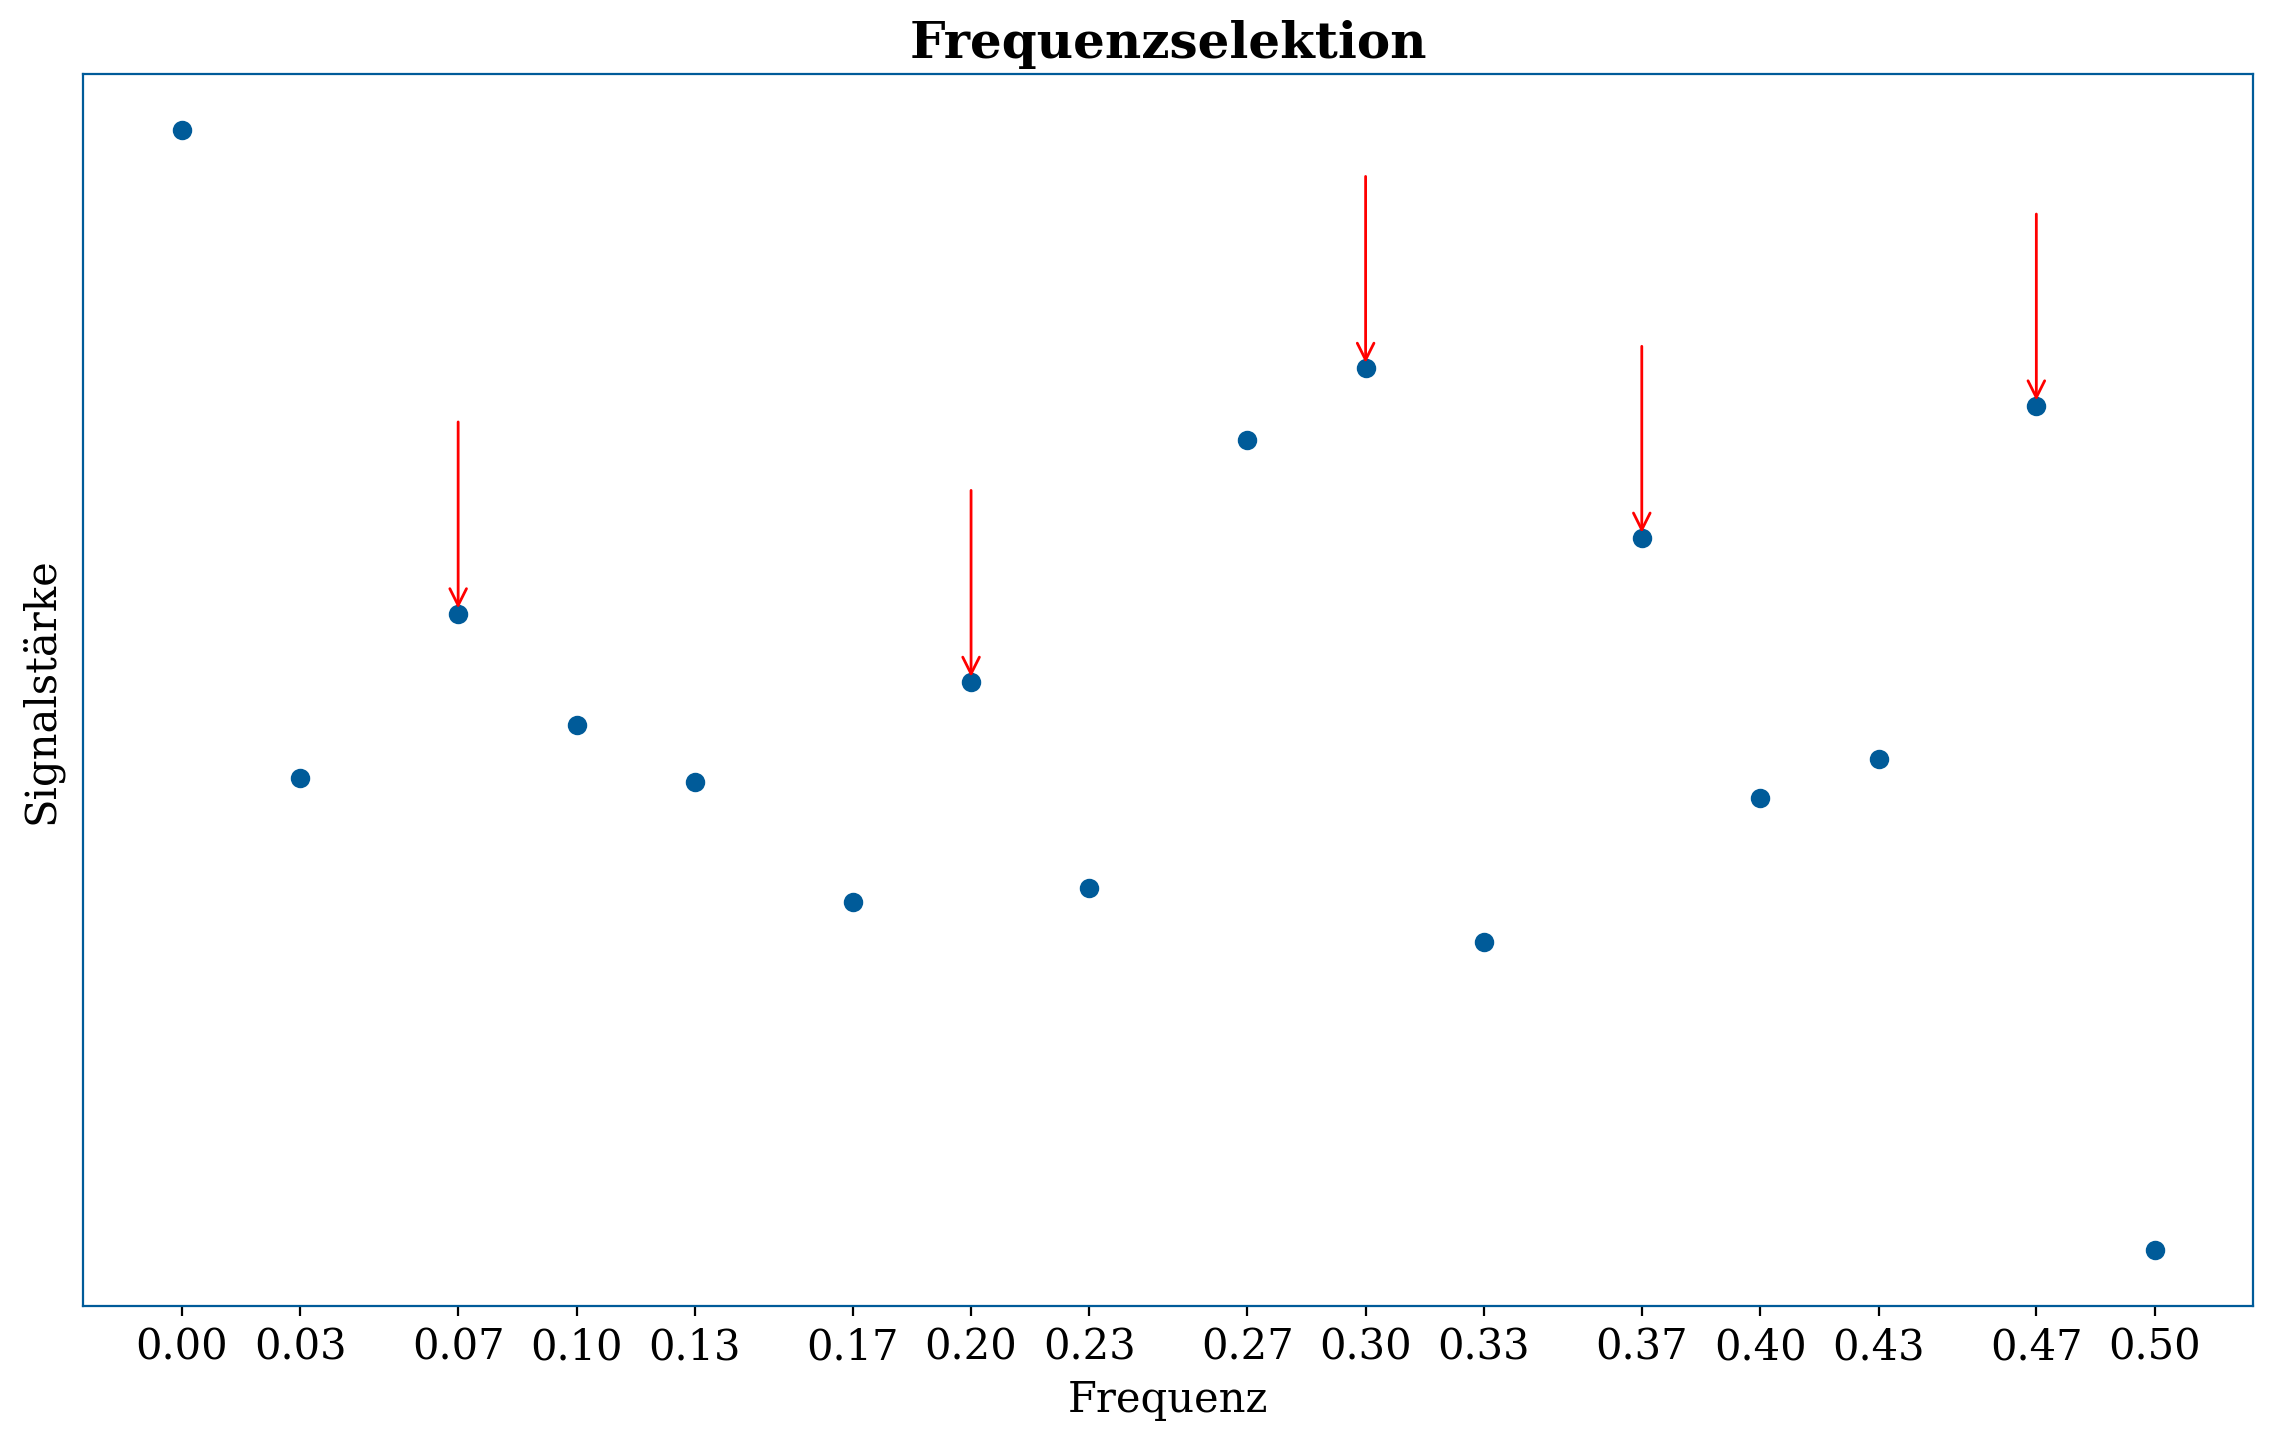
\includegraphics[width=0.5\textwidth]{plot_frequency_selection.png}
        \caption{Spektralanalyse eines Fensters der STFT mit Markierung lokaler Maxima}
        \label{fig:freq_selection}
    \end{wrapfigure}

    In \autoref{fig:freq_selection} wird dieser Sachverhalt für ein Fenster der STFT dargestellt. Es werden die Signalstärken für alle möglichen Frequenzen ermittelt, wobei das Reziproke einer Frequenz hier entspricht, jedes wievielte Element betrachtet wird. Bei Frequenz 0.5 wäre es also jedes $\frac{1}{0.5} = 2$te Element, hier offenbar sehr schwach ausgeprägt. Diese Signalstärke oder Amplitude der Frequenz wird über Summen der Originaldaten ermittelt. Frequenz 0 ist lediglich die Summe aller Eingabewerte, also hier allen Kidera-Fakor-Werten, die den numerischen Vektor der Eingabe-Aminosäurekette darstellten.

    Damit die Musikerkennung funktioniert, wird nun vorher eine Datenbank erstellt, welche die Periodizitäten der Eingabesongs mittels Hashing effizient auffindbar abspeichert, sodass der Abgleich mit einer Tonaufnahme sehr schnell und korrekt abläuft \vgl{wang}. Zudem werden hierfür aus den STFT-Ergebnissen auch nicht alle Frequenzen verwendet, sondern nur möglichst signifikante davon. Bisher wird das mittels der lokalen Maxima der Amplituden erreicht.

    Für die Anwendung auf Proteine werden statt des musikalischen Spektrums die numerischen Vektoren der Aminosäuresequenzen verwendet. Nun gibt es in \protfin\ zwei verschiedene Anwendungsansätze:
    \begin{enumerate}
        \item \textbf{Single-Protein:}\ \ Als Eingabe erfolgt eine einzelne Aminosäuresequenz, für die das best passende Protein gesucht wird. Je mehr Übereinstimmung herrscht, desto funktionsähnlicher sollte es sein.
        \item \textbf{Family-Matching:}\ \ Als Eingabe erfolgt eine Proteinfamilie. Die Periodizitäten, in denen sich alle Mitglieder dieser Familie ähneln, die also spezifisch für die Familie sind, werden verwendet, um Proteine zu finden, die auch in die Familie passen.
    \end{enumerate}
    Um den Algorithmus für beide Ansätze auf die vergleichsweise kurzen Sequenzen von wenigen 100 Elementen abzustimmen (ein solcher Vektor für eine Sekunde Musik hätte etwa 40.000 Elemente), wurde in vorangegangenen Experimenten versucht, die Fenstergröße und die Überlappung zwischen diesen Fenstern bei der STFT zu optimieren, beziehungsweise auch die Anzahl gewählter Frequenzen, deren Amplituden auf Periodizität hindeuten. Hierbei zeigte sich allerdings eine schlechte Performanz hinsichtlich Speicher- und Laufzeitkomplexität. Die Wahl der Frequenzen der STFT Fenster und deren Abspeicherung müssen folglich noch verbessert werden.

    Hierzu werden in dieser Arbeit mehrere Experimente angegangen.
    \begin{enumerate}
        \item \textbf{UniRef90-Sampling:}\ \ Je weniger Frequenzen in einem Fenster ausgewählt werden, desto weniger muss gespeichert werden. In diesem Experiment werden solche Fenster aus der UniRef90 Datenbank gesampelt. Sie enthält etwa 180 Mio. Aminosäuresequenzen, sodass aus jeder ein zufälliges Fenster gewählt wird. Die je Frequenz seltensten Amplituden sollen nun als Schwellwert das Wahlkriterium für eine Frequenz sein, was zu möglicherweise weniger selektierten Frequenzen mit dennoch guter Signifikanz führt.
        \item \textbf{Filter Hashes:}\ \ Ein weiterer Ansatz die Datenbankgröße zu verringern ist das Entfernen von Hashes, die sehr häufig auftreten, also folglich wenig Informationsgehalt für die Identifikation eines Proteins haben. In diesem Experiment wird daher geprüft, wie streng das erfolgen darf, um nicht zu viel Daten zu verlieren, sodass das Matching dadurch beeinträchtigt würde. 
        \item \textbf{\acl{TZ}:}\ \ Die effiziente Abspeicherung mittels Hashing basiert darauf, die Frequenzen eines Fensters mit den Frequenzen der Nachfolgefenster zu kombinieren. Die \acl{TZ} bezeichnet dabei die Anzahl betrachteter Nachfolger und ist aktuell unbeschränkt. Folglich wird hier eine Größe ermittelt, die einen guten Kompromiss zwischen der Anzahl an Kombinationen und der Genauigkeit des Matchings bildet.
        \item \textbf{Selection-Method:}\ \ Das letzte durchgeführte Experiment dieser Arbeit dient der Ermittlung einer Methode für die Frequenzselektion, die vom UniRef90-Sampling profitiert, aber die Auswahl zusätzlich reduziert. Dafür wird vor Betrachtung der Schwellwerte eine Vorselektion durchgeführt, einmal anhand der lokalen Maxima der Amplituden, dann anhand der stärksten Abweichungen der Amplituden von ihren Schwellwerten und natürlich ohne Vorselektion als Nullprobe, die nur das Sampling einbezieht. Dabei wird die Datenbankerstellung abgebrochen, sobald deren Größe die Eingabe um ein 6-faches übersteigt.
    \end{enumerate}
    Als Trainingsdaten wird eine Referenz-Datenbank von Pflanzen-Proteinen verwendet, die in Gruppen derselben Funktion eingeordnet sind. Diese Zuordnung wurde manuell von Experten durchgeführt in sogenannte MapMan-Bins, was heißt:\\Derselbe Bin $\rightarrow$ dieselbe Funktion \cite{mapman}.

    \textit{Diese Bachelorarbeit ist auf GitHub\footnote{\url{https://github.com/qwerdenkerXD/Bachelorarbeit-Bioinformatik}} verfügbar. Bei Fragen oder Anmerkungen zur Kontaktaufnahme bitte die dortige Issue-Funktion verwenden.}
% section einleitung (end)